
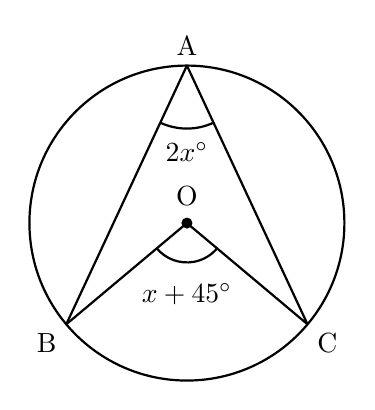
\begin{tikzpicture}[scale=1]

    % Define the center of the circle and points on the circumference
    % O is the center, A is at the top, B and C are placed symmetrically
    \coordinate (O) at (0,0);
    \coordinate (A) at (90:2);
    \coordinate (B) at (220:2);
    \coordinate (C) at (320:2);

    % Draw the main outer circle
    \draw[thick] (O) circle (2cm);

    % Draw the chords AB and AC forming the inscribed angle
    \draw[thick] (A) -- (B);
    \draw[thick] (A) -- (C);

    % Draw the radii OB and OC forming the central angle
    \draw[thick] (O) -- (B);
    \draw[thick] (O) -- (C);

    % Mark the center point O with a small filled dot
    \fill (O) circle (2pt);

    % Draw the arc for the inscribed angle BAC
    % The angle is centered around 270 degrees (downward), spanning 50 degrees total (245 to 295)
    \draw[thick] (A) ++(245:0.8) arc (245:295:0.8);

    % Place the label for angle BAC
    \node at (0, 0.9) {$2x^\circ$};

    % Draw the arc for the central angle BOC
    % The angle spans from 220 degrees to 320 degrees
    \draw[thick] (O) ++(220:0.5) arc (220:320:0.5);

    % Place the label for angle BOC
    \node at (0, -0.9) {$x + 45^\circ$};

    % Add the labels for the points A, B, C, and O
    \node[above] at (A) {A};
    \node[below left] at (B) {B};
    \node[below right] at (C) {C};
    \node[above] at (0, 0.1) {O};

\end{tikzpicture}